% Level ceiling (grade 6): density handled as "mass of one cubic
% centimetre" via proportionality tables and division; the literal
% formula rho = m/V waits for grade 7 (literal expressions, math g7).
\chapter{密度：为什么物体会漂浮}\label{ch:g6:density-floating}

在你刚入学的第一年，一枚小硬币沉了下去，而一根大木头却浮了起来，
我们曾承诺，“为什么”正是本课程的宝藏。
你已经赢得了它。钥匙是在前两章里锻造成的，
物质看质量，房间看体积 --- 今天这两者
在这把锁上合力转动。

\section{一立方厘米的质量}

\begin{example}[终于可以公平比较]\label{ex:g6:density-floating:fair}
把整根木头和整枚硬币放在一起比，从来都不公平：
大小不同，形状也不同。公平的比赛应当取\emph{相同
体积}：每位参赛者各取一立方厘米。
一 \unit{cm^3} 水的质量为 \qty{1}{g}；一 \unit{cm^3}
的橡木约 \qty{0.6}{g}；石头约 \qty{2.5}{g}；
铁为 \qty{7.9}{g}。空间相同，物质却千差万别 --- 这正是
浮沉游戏一直在等待的那个数字。
\end{example}

\begin{definition}[密度]\label{def:g6:density-floating:density}
某种物质的\emph{密度}\index{密度}，是指
该物质一立方厘米的质量，单位为克。水的密度是
\qty{1}{g} 每 \unit{cm^3}；橡木约 $0.6$；铁为 $7.9$。求
密度不需要新仪器：只需测出样品的
质量和体积，然后相除 --- 把克数平均分给各立方厘米，
答案便是每立方厘米所得的
份额。
\end{definition}

\begin{omfigure}
\begin{tikzpicture}[scale=0.85]
  \foreach \x/\name/\m/\c in {0.9/软木/0.2/omMeth,
      3.0/橡木/0.6/omMeth, 5.1/水/1.0/omDef,
      7.2/石头/2.5/omExo, 9.3/铁/7.9/omThm} {
    \draw[thick, fill=\c, fill opacity=0.4]
      (\x,0.6) rectangle ++(1.0,1.0);
    \node[above, font=\footnotesize] at (\x+0.5,1.65) {\name};
    \node[below, font=\footnotesize] at (\x+0.5,0.5)
      {$\m$ g};
  }
  \node[below, font=\small] at (5.6,-0.15)
    {五块相同的一立方厘米方块 --- 五种质量};
\end{tikzpicture}

{\small 公平的比赛：每人空间相同，每种
物质都显出自己的“特征质量”。}
\end{omfigure}

\begin{proposition}[密度是特征]\label{prop:g6:density-floating:signature}
纯净物质的密度，对其任一部分都相同，
无论大小：一小块橡木和一整根横梁，都是
每立方厘米约 \qty{0.6}{g}。因此，密度可以识别物质，
与熔点一样：测出一个不明物体的
质量和体积，相除后与表格对照 ---
物质往往当场就能“招供”。
\end{proposition}

\begin{method}[测量密度]\label{met:g6:density-floating:measure}
对于一块卵石 --- 或一顶王冠：
\begin{enumerate}
  \item 用天平测出它的质量，比如 \qty{75}{g}；
  \item 用水面上升法测出它的体积，比如
        \qty{30}{cm^3};
  \item 把克数除以立方厘米数：$75 \div 30 =
        2.5$ --- 每立方厘米含 \qty{2.5}{g}；
  \item 查表：密度为 $2.5$ --- 这块卵石是
        普通的石头。
\end{enumerate}
\end{method}

\section{浮沉规律}

\begin{proposition}[物体为什么会漂浮]\label{prop:g6:density-floating:rule}
物体在水中漂浮，若其密度\emph{小于}
水的密度 --- 即每立方厘米不足 \qty{1}{g} ---，
若密度更大则下沉。可以说，水在把闯入者与自身
逐体积地比较：每单位体积比水轻的浮在上面；
每单位体积比水重的则沉下去。同样的规律适用于
任何液体，各自以其密度作为裁判。
\end{proposition}

\begin{omfigure}
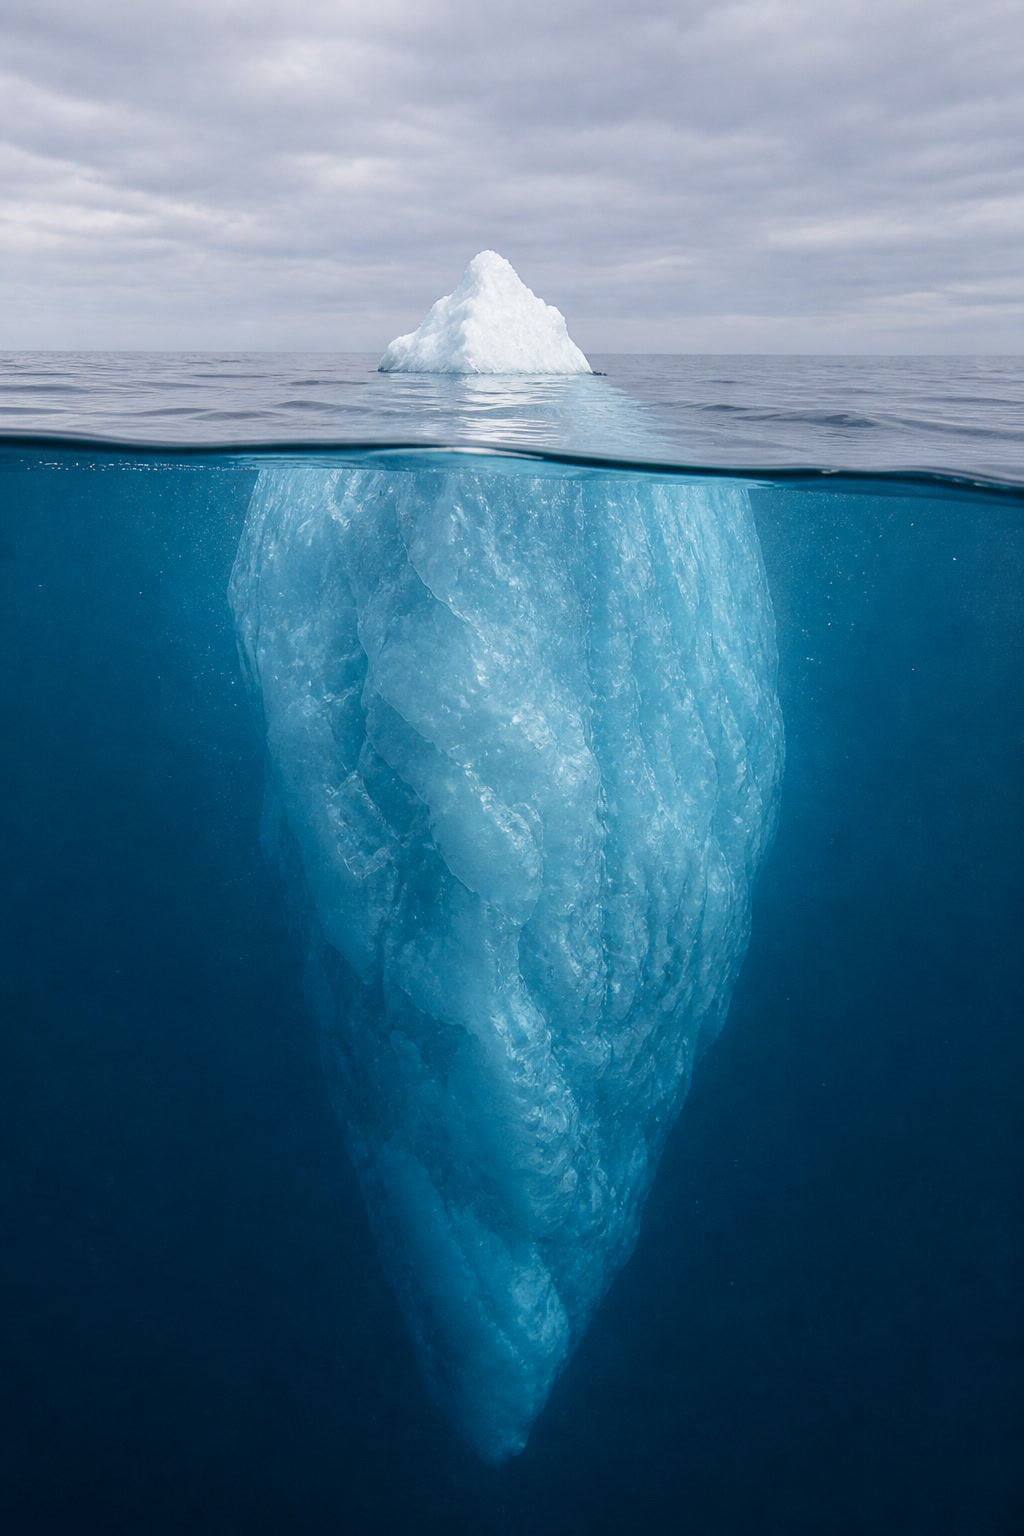
\includegraphics[width=0.4\linewidth]{images/book1/ai/g6-density-iceberg.jpg}

{\small 冰的密度只略小于水 --- 因此冰山漂浮时，大部分体积隐藏在水面以下。}
\end{omfigure}

\begin{example}[六年谜题，终于解开]\label{ex:g6:density-floating:settled}
木头（$0.6$）：无论多大都会漂浮 --- 它的每立方厘米
都比水轻。硬币（青铜，约 $9$）：无论多小都会
下沉。塑料鸭、软木塞、铅笔：密度都在 $1$ 以下，
统统是漂浮者。冰，密度为 $0.9$ --- 水自己膨胀后的固体 ---
在自身的液体上勉强浮着，只差一丝，所以池塘常盖着
冰盖，冰山才能漂航。那么橡皮泥小船呢？做成
碗形，\emph{船加空气}这一整体单位体积内含空气很多：
整体的密度降到 $1$ 以下，而在码头上，
同样的诀窍让一艘艘万吨钢船下水。
\end{example}

\begin{omfigure}
\begin{tikzpicture}[scale=0.85]
  \draw[thick] (0.8,0) -- (0.8,3.4) (4.0,0) -- (4.0,3.4)
    (0.8,0) -- (4.0,0);
  \fill[omMeth, opacity=0.35] (0.8,2.2) rectangle (4.0,3.0);
  \node[font=\footnotesize] at (2.4,2.6) {油：$0.9$};
  \fill[omDef, opacity=0.3] (0.8,1.1) rectangle (4.0,2.2);
  \node[font=\footnotesize] at (2.4,1.65) {水：$1.0$};
  \fill[omThm, opacity=0.3] (0.8,0.05) rectangle (4.0,1.1);
  \node[font=\footnotesize] at (2.4,0.55) {蜂蜜：$1.4$};
  \node[below, font=\small] at (2.4,-0.3)
    {液体分层：底部密度最大};
  \draw[thick] (7.2,0) -- (7.2,3.4) (11.0,0) -- (11.0,3.4)
    (7.2,0) -- (11.0,0);
  \fill[omDef, opacity=0.3] (7.2,0.05) rectangle (11.0,2.6);
  \draw[thick, fill=white]
    (8.3,2.35) -- (9.9,2.35) -- (9.6,2.95) -- (8.6,2.95) -- cycle;
  \draw[thick, fill=white, fill opacity=0.7]
    (8.0,2.35) -- (10.2,2.35) -- (9.5,1.0) -- (8.7,1.0) -- cycle;
  \node[font=\footnotesize] at (9.1,1.85) {冰：$0.9$};
  \node[below, font=\small] at (9.1,-0.3)
    {冰山：十分之九在水面以下};
\end{tikzpicture}

{\small 密度的“笔迹”：液体按密度由大到小自下而上分层，
冰（$0.9$）浮在水面上时，仅十分之一露出水面。}
\end{omfigure}

\begin{example}[液体塔]\label{ex:g6:density-floating:tower}
先把蜂蜜，再把染了墨的水，最后把油，沿着高玻璃杯的内壁轻轻倒入，
形成三层：蜂蜜（$1.4$）在底部，油
（$0.9$）在顶部，它们各守层次，互不相混。放入几位“客人”：一颗
葡萄（$1.05$）先穿过油下沉，再穿过水下沉，
最后停在蜂蜜层上——它比油和水都密，却比蜂蜜轻。
这座“液体塔”把浮沉规律演成了一出戏。
\end{example}

\begin{remark}[读懂冰山]\label{rem:g6:density-floating:iceberg}
冰的 $0.9$ 与水的 $1.0$ 相比，不仅使冰山浮起，
它还决定了水线的位置。冰山十分之九的体积位于
\emph{水面以下}——正是那块隐藏的质量，
曾使不少自负的船只沉没。水下部分的比例究竟\emph{为何}恰好等于
密度之比，这是一条优美的定律，由阿基米德
本人发现，其严格证明将在高中分册中给出；
密度表已经暗示了答案。
\end{remark}

\section{王冠，终于揭晓}

\begin{example}[阿基米德破案]\label{ex:g6:density-floating:crown}
现在来讲完两章前开始的故事。王冠的质量：
容易，天平即可测得。它的体积：对于形状不规则的
工艺品而言难以直接测量——直到“澡盆”的启示给出了排水法。
质量除以体积：王冠的\emph{密度}——
而密度就是一种“指纹”。纯金的为 $19.3$；白银的为
$10.5$；某种秘密配比的合金则介于两者之间。传说
金匠的王冠“招认”出的密度远低于纯金，
骗局就此被揭穿，王冠却毫发无损。
周末问题给出了他的数据。
\end{example}

\section{练习}

\begin{exercise}[$\star$]\label{exo:g6:density-floating:1}
什么是物质的密度？写出水的密度，并叙述
浮沉规律。
\end{exercise}

\begin{exercise}[$\star$]\label{exo:g6:density-floating:2}
预测下列物体放入水中是上浮还是下沉：橡木（$0.6$）；\ 石头（$2.5$）；\
软木（$0.2$）；\ 铁（$7.9$）；\ 冰（$0.9$）。
\end{exercise}

\begin{exercise}[$\star$]\label{exo:g6:density-floating:3}
一块物体的质量为 \qty{120}{g}，体积为 \qty{80}{cm^3}。求它的
密度，它放入水中会上浮还是下沉？
\end{exercise}

\begin{exercise}[$\star$]\label{exo:g6:density-floating:4}
一块神秘的物块：质量为 \qty{158}{g}，放入量筒后液面上升
\qty{20}{cm^3}。求它的密度，并根据本章的数据，
推断它可能是哪种物质？
\end{exercise}

\begin{exercise}[$\star$]\label{exo:g6:density-floating:5}
为什么一小块橡木的密度与整根橡木梁
的密度相同？这一性质有什么用处？
\end{exercise}

\begin{exercise}[$\star$]\label{exo:g6:density-floating:6}
在液体塔中，为什么蜂蜜在最下面，油在
上面？密度为 $1.05$ 的葡萄会停在哪里？
\end{exercise}

\begin{exercise}[$\star$]\label{exo:g6:density-floating:7}
冰能浮在水面上——对于固体来说，这为什么是反常的？
哪一条关于水凝固的古老命题可以解释冰的 $0.9$？
\end{exercise}

\begin{exercise}[$\star$]\label{exo:g6:density-floating:8}
七年级时学过的“大木头”和“小硬币”：给出
最终、完整的答案，并利用本章的数据。
\end{exercise}

\begin{exercise}[$\star\star$]\label{exo:g6:density-floating:9}
某种液体一升的质量为 \qty{800}{g}。以克每立方厘米为单位，它的
密度是多少？一块冰块
（$0.9$）放入其中会上浮还是下沉？
\end{exercise}

\begin{exercise}[$\star\star$]\label{exo:g6:density-floating:10}
钢的密度为 $7.9$，但钢船却能浮在水面上。请运用
借助
\cref{ex:g6:density-floating:settled}中的“包裹”思想——除了钢，船上的“包裹”还包括什么，
以及其整体密度必须为多少？
破损的船何时不再满足这一规律？
\end{exercise}

\begin{exercise}[$\star\star$]\label{exo:g6:density-floating:11}
海水的密度比淡水略大，约为 $1.03$。
解释为什么人在海水中漂浮得明显更好，并预测
一艘船从咸海驶入淡水河时，
其水线会如何变化。
\end{exercise}

\begin{exercise}[$\star\star\star$]\label{exo:g6:density-floating:12}
一个空心金属球恰好有一半浸在水中漂浮。
推算\emph{整个球形“包裹”}（金属
外壳加内部空气）的密度。然后论证，若水缓慢渗入
球内，它会向哪个方向运动，并说明在什么时刻开始下沉
——请同时运用规律与“包裹”的思想。
\end{exercise}

\section{周末问题：国王的王冠}

\begin{problem}[{周末问题 --- 国王王冠一案，
用你的仪器重新审视；金匠的审判，
借除法破解}]\label{pb:g6:density-floating:1}
用现代数据重新审视古代最著名的欺诈案。
特征数据：金 $19.3$，银 $10.5$（
克每立方厘米）。

\medskip\noindent\textbf{第一部分 --- 证据。}
国王交给金匠 \qty{1930}{g} 纯金。
做成的王冠放在天平上，质量恰好为 \qty{1930}{g}。
\begin{enumerate}
  \item 质量完全吻合。为什么仅凭这一点
        无法说明任何欺诈问题？（金匠能做什么，
        仍能使质量吻合？）
  \item \qty{1930}{g} 的 \emph{纯金}应占多大体积？
        （把克数分组：每组
        \qty{19.3}{g}，可占几立方厘米？）
  \item 阿基米德将王冠放入盛满水的容器中，
        收集溢出的水，其体积为 \qty{130}{cm^3}。
        王冠的真实体积是多少？
  \item 比较两个体积。这一比较已经
        说明了什么？
\end{enumerate}

\medskip\noindent\textbf{第二部分 --- 特征数据。}
\begin{enumerate}[resume]
  \item 由王冠的质量和测得的体积，
        计算王冠的密度（保留一位小数即可）。
  \item 将三个特征数据并列比较：金、王冠、
        银。王冠的密度落在何处？
  \item 用一句话向国王解释，王冠为何
        不可能是纯金。
  \item 金匠抗议：“也许是天平出错了！”
        姑且给他宽限，允许天平向任一方向有 \qty{30}{g} 的误差。
        在 \qty{1900}{g} 与 \qty{1960}{g} 之间，
        能否使体积为 \qty{130}{cm^3} 的纯金王冠得以“开脱”？
        （请检验密度范围。）
\end{enumerate}

\medskip\noindent\textbf{第三部分 --- 究竟偷了多少？}
假设金匠私吞了一部分黄金，并以银按
同样的克数予以替换。
\begin{enumerate}[resume]
  \item 以银替换金，按相同克数替换，
        质量仍然正确，体积却为何会\emph{膨胀}？
  \item 检验一个猜想：一顶王冠由 \qty{965}{g} 金 $+$
        \qty{965}{g} 银组成。金的部分体积是多少？
        银的部分体积是多少？（保留一位小数。）
  \item 求出猜想中王冠的总体积，并以
        实测的 \qty{130}{cm^3} 检验此猜想：银是多了，还是
        少了？
  \item 法庭需要一句判决：陈述已被毫无疑问证明的
        结论（是否为纯金），所用的方法是什么，
        以及王冠为何无需受损 ——
        这正是阿基米德真正的胜利。
\end{enumerate}
\end{problem}
